% arara: indent: {overwrite: yes}
\section{Лабораторная 4}

\subsection{Условие}

\textbf{Согласно варианту 10:}
\begin{enumerate}
	\item $I_{1} = \int\limits_{-\infty}^{\infty} e^{-x^{4} \sqrt{1+x^{4}}} dx$;
	\item $I_{2} = \iint\limits_{1 \leqslant x^{2} + y^{2} \leqslant 4} \frac{dxdy}{x^{2} + y^{2}}$.
\end{enumerate}

Вычислить значение интеграла, используя метод Монте-Карло. Оценить точность.

\begin{enumerate}
	\item По методу Монте-Карло вычислить приближённое значение интегралов;
	\item Сравнить полученное значение либо с точным значением (если его получится вычислить), либо с приближённым, полученным в каком-либо математическом пакете (например, в mathematica). Для этого построить график зависимости точности вычисленного методом Монте-Карло интеграла от числа итераций $n$.
\end{enumerate}

\subsection{Теория}
\subsubsection{Метод Монте-Карло для вычисления интегралов}

В основе метода лежит нахождение такой случайно величины $\xi$, математическое ожидание которой совпадает с искомым интегралом:

\begin{equation}
	\int\limits_{a}^{b}f(x)dx = E(\xi) = \int\limits_{a}^{b}x\rho_{\xi}(x)dx.
\end{equation}

Для этого выбирается такая СВ $\xi_{1}$ с плотностью $\rho_{\xi_{1}}(x)$, определённая на той же области, что и интеграл, тогда $\xi$ определяется, как

\begin{equation}
	\xi = g(\xi_{1}) = \frac{f(\xi_{1})}{\rho_{\xi_{1}}(\xi_{1})}.
\end{equation}

Тогда

\begin{equation}
	E(\xi) = E(g(\xi_{1})) = \int\limits_{a}^{b}g(x)\rho_{\xi_{1}}(x)dx = \int\limits_{a}^{b}\frac{f(x)}{\rho_{\xi_{1}}(x)}\rho_{\xi_{1}}(x)dx = \int\limits_{a}^{b}f(x)dx.
\end{equation}

Для нахождения математического ожидания необходимо смоделировать $n$ реализаций $x_{i}$ СВ $\xi$:
\begin{equation}
	E(\xi) \approx \frac{1}{n} \sum\limits_{i=0}^{n}x_{i}.
\end{equation}

\paragraph{Алгоритм моделирования:}\
\

\begin{enumerate}
	\item Для вычисления $I_{1}$ использовалось нормальное распределение $N(0,1)$, область которого совпадает с областью интегрирования;
	\item При вычислении $I_{2}$ производился переход к полярной системе координат и использовать равномерное распределение на отрезке [0, 2].
\end{enumerate}

\subsection{Код программы}

\lstinputlisting[language=Python]{./lab_4/lab4.py}

\subsection{Результат выполнения}

\begin{figure}[H]
	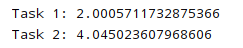
\includegraphics {results_lab_4.png}
	\label{fig:results_lab_1}
	\caption{Результат выполнения программы: значения интегралов $I_{1}, I_{2}$ соответственно.}
\end{figure}

\begin{figure}[!h]
	\centering
	\begin{subfigure}[b]{0.45\textwidth}
		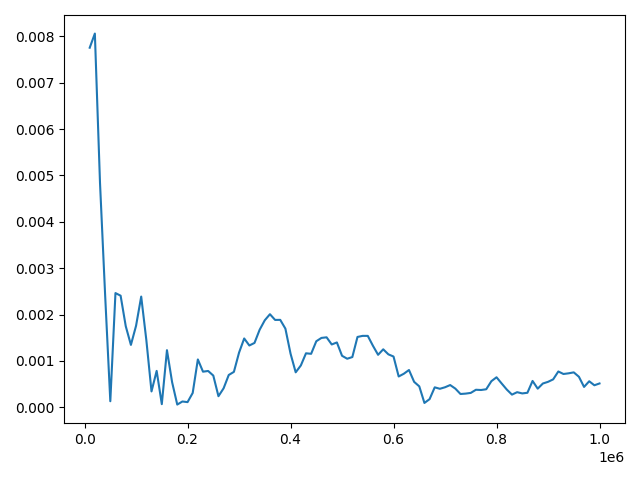
\includegraphics[width=\textwidth]{integral_discrepancies.png}
		\caption{График зависимости точности вычисленного методом Монте-Карло интеграла $I_{1}$ от числа итераций $n$.}
	\end{subfigure}
	\hfill
	\begin{subfigure}[b]{0.45\textwidth}
		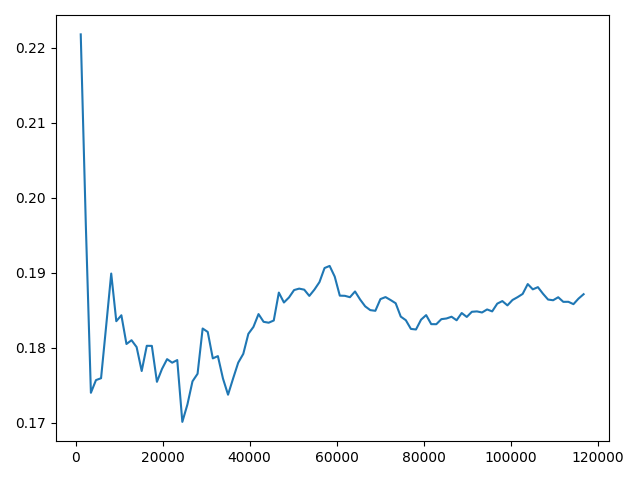
\includegraphics[width=\textwidth]{double_integral_discrepancies.png}
		\caption{График зависимости точности вычисленного методом Монте-Карло интеграла $I_{2}$ от числа итераций $n$.}
	\end{subfigure}
\end{figure}
